% !TEX TS-program = Xelatex
% !TEX encoding = UTF-8 Unicode

\documentclass[UTF8]{ctexart}
\usepackage{amsmath}
\usepackage[bottom]{footmisc}
\usepackage{geometry}
\usepackage{graphicx}
\usepackage{figsize}
\usepackage[separate-uncertainty = true,per-mode=symbol]{siunitx}
\usepackage{tabu}
\usepackage{wasysym}
\geometry{left=0.7in,right=0.7in,bottom=0.7in,top=0.7in}

\title{实验十五:非平衡电桥测Pt100的温度系数}
\author{朱寅杰 1600017721}
\date{2017年11月10日}

\begin{document}

\maketitle

实验使用恒流源,电流为$I=\SI{4.006}{\milli\ampere}$。$R_p=\SI{100.2}{\ohm}$。测到的$U$随温度$t$的变化如下表。
\begin{center}
\begin{tabu} to \linewidth {X[c]|X[c] X[c] X[c] X[c] X[c] X[c] X[c]}
\hline
$t/\si{\celsius}$	&0.1	&21.2	&44.4	&56.8	&71.5	&85.6	&100.1
\\
\hline
$U/\si{\milli\volt}$	&0.00	&16.02	&33.80	&43.32	&54.37	&65.05	&76.07
\\
\hline
\end{tabu}
\end{center}

\begin{figure}[h]
  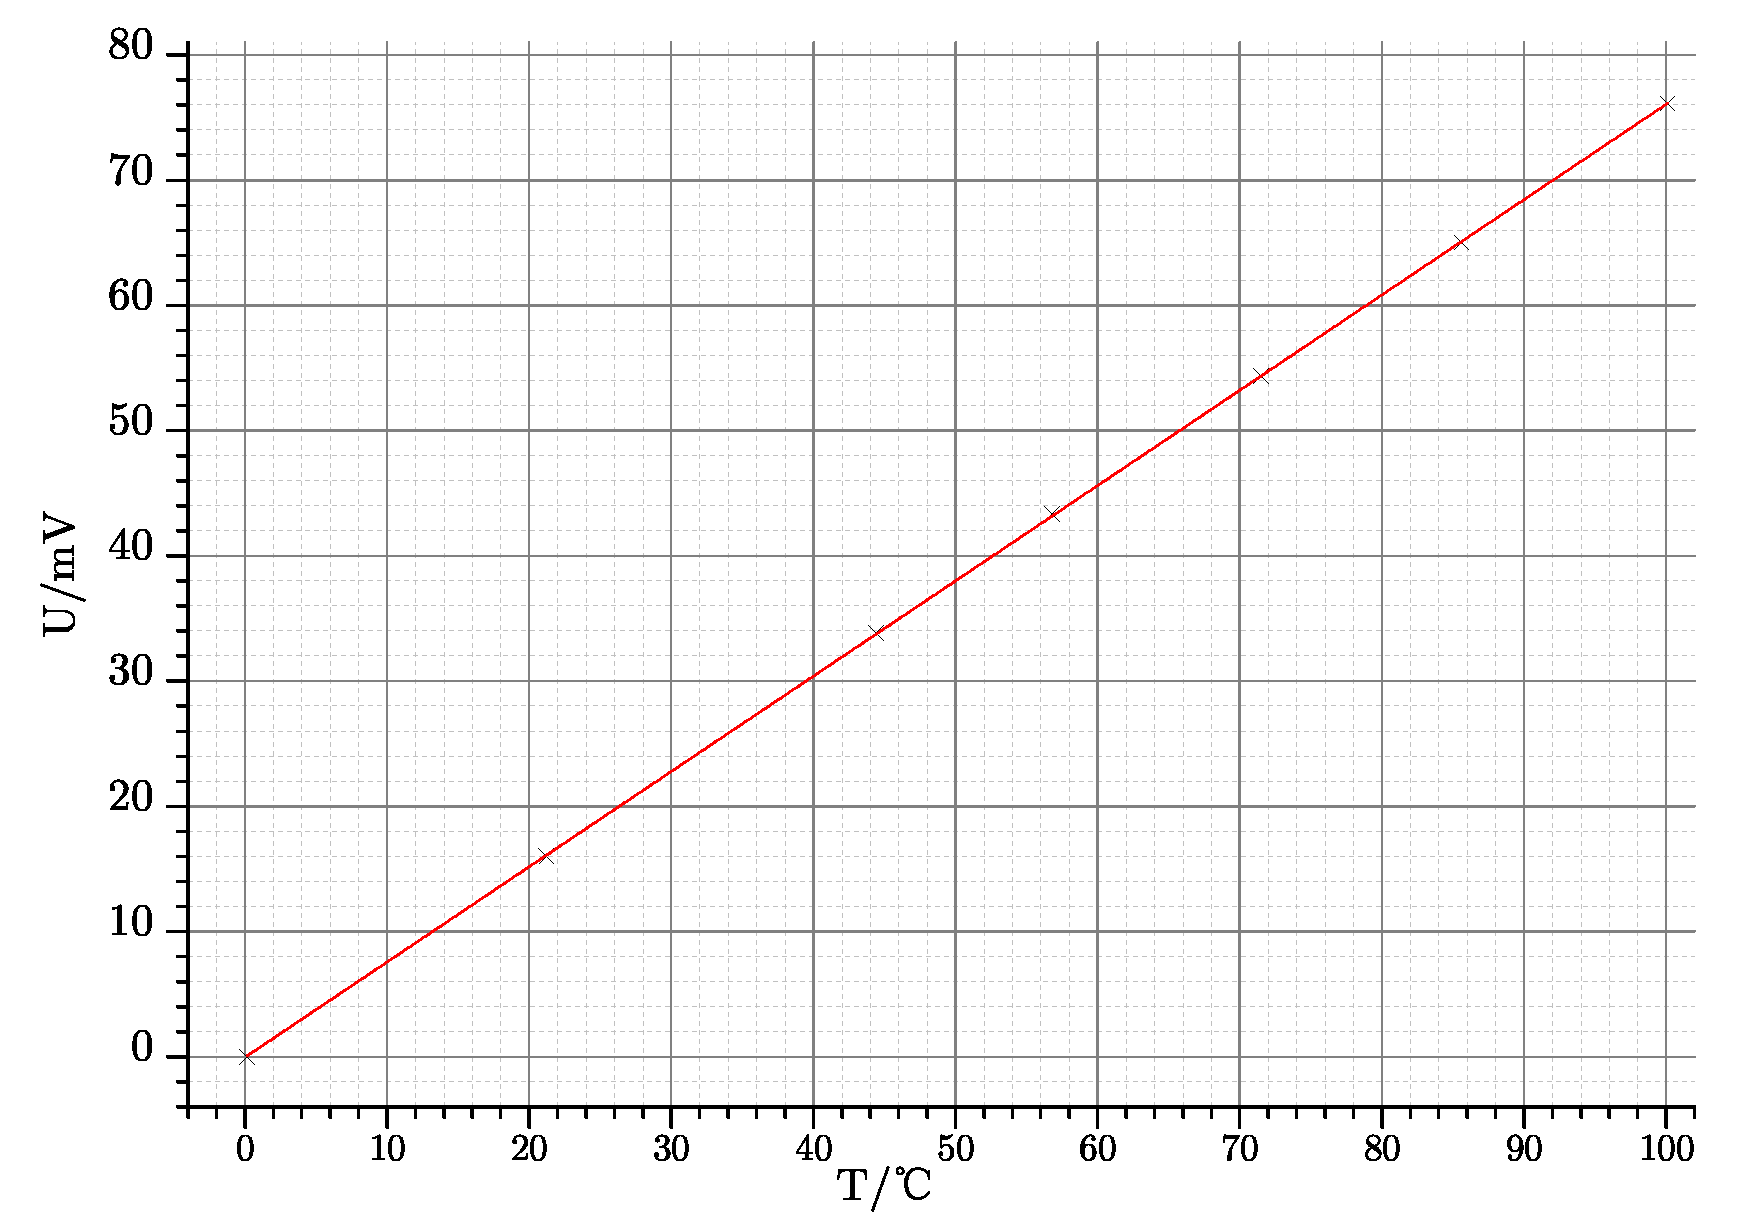
\includegraphics[width=\linewidth,keepaspectratio=true]{Pt100.eps}
  \caption{$U-t$关系图。}
\end{figure}
对表中数据作线性拟合得到
\begin{equation}
  U=\SI{.04}{\milli\volt}+\SI{.7609}{\milli\volt\per\celsius}\times t
\end{equation}
$r=\num{.999996}$
因此斜率的不确定度有$\sqrt{(1/r^2-1)/(N-2)}=\SI{9.6e-4}{\milli\volt\per\celsius}$。测量电压所用万用表有0.05\%+3个字,相当于约\SI{.13}{\milli\volt}的允差,折算成相对不确定度约是千分之二,两者按方和根合成得$\Delta U/\Delta t$的相对不确定度为\num{2.2e-3}。电流档有0.5\%+4个字的允差,故对电流的测量约有\SI{.024}{\milli\ampere}的允差,折成标准差有$I=\SI{4.006(14)}{\milli\ampere}$,其相对不确定度为\num{3.5e-3}。电阻箱读数为\SI{100.2}{\ohm},\SI{100}{\ohm}档允差0.1\%,0.1欧允差2\%,因此其允差约为\SI{0.1}{\ohm}。故$R_p$的相对不确定度有\num{5.8e-4}。



温度系数$A_1=\frac{2}{IR_p}\frac{\Delta U}{\Delta t}$,故$A_1$的相对不确定度为以上三项的方和根为\num{4.2e-3},有$A_1=\SI{3.79(2)e-3}{\per\celsius}$
\section*{思考题}
\paragraph{线性的保证}
实验中$R_1$与$R_2$取得远大于Pt100的电阻,并且使用内阻极大的数字万用表使得电桥上电压对于铂电阻的响应足够线性。同时采用恒流源而非恒压源,简化计算的同时保证电流不变也能保证响应足够地线性。测量时所用的温度范围不太大,在铂电阻本身的线性范围之内。以上几个因素共同保证了实验中各环节的响应是足够线性的。
\paragraph{截距的影响}
纯从理论说,如果在冰水混合物中电桥给调平衡了,那么截距不为零就肯定是温度计零点不在冰水混合物的零度,这对于最终的测量结果并没有太大的影响。从实际上讲,即便是非常好的线性关系,从统计上也能计算出截距有着一个很大的不确定度(比如本次实验回归出的截距及其统计不确定度为\SI{.04(6)}{\milli\volt}),再加上仪器自身的允差,可以看出这貌似非零的截距早就被淹没在不确定度里了,对此挖空心思实在是毫无意义。
\end{document}